\documentclass{jfm}

\usepackage{xcolor}
\usepackage{array}
\usepackage{longtable}

\usepackage{graphicx,color}
% \usepackage[section]{placeins}
\usepackage{float}
% \usepackage{graphicx,subfigure}
\usepackage{subcaption}
\usepackage{epstopdf, epsfig}
\usepackage{amstext}
\usepackage{amsmath}
\usepackage{todonotes}
\usepackage{hyperref}
\usepackage{verbatim}
\usepackage{bm}
\usepackage{diagbox}
\usepackage{forloop}

\usepackage{listings}
\usepackage[numbered,framed]{matlab-prettifier}
% \let\ph\mlplaceholder % shorter macro
% \lstMakeShortInline"

\lstset{
  style              = Matlab-editor,
  basicstyle         = \mlttfamily,
  escapechar         = ",
  mlshowsectionrules = true,
}

\newtheorem{theorem}{Theorem}
\newtheorem{defn}{Definition}
\newtheorem{lemma}{Lemma}
\newtheorem{corollary}{Corollary}
\newtheorem{prop}{Proposition}
\newtheorem{assume}{Assumption}
\newtheorem{notation}{Notation}
\DeclareMathOperator*{\argmin}{arg\,min}

\newcommand\nc{\newcommand}
\nc\qu{\quad}
\nc\tends{\rightarrow}
\nc\dint{\int\!\int}
\newcommand{\vect}[1]{\mbox{\boldmath $#1$}}
\nc{\degree}{\mbox{\footnotesize{o}}}

\newcommand{\bes} {\begin{eqnarray*}}
\newcommand{\ees} {\end{eqnarray*}}
\newcommand{\dd} \partial

\newcommand{\non} \nonumber
\newcommand{\ie}{{\it i.e.}\ }
%\newcommand{\eg}{{\it e.g.}\ }
%\newcommand{\etal}{{\it et al.} \ }
\newcommand{\ru}{R_{\rm u}}
\newcommand{\rb}{R_{\rm b}}
\newcommand{\qup}{Q_{\rm u,pore}}
\newcommand{\qbp}{Q_{\rm b,pore}}

\newcommand{\ra}{\rightarrow}

\nc\cA{{\cal{A}}}
\nc\cB{{\cal{B}}}
\nc\cZ{{\cal{Z}}}
\nc\cX{{\cal{X}}}
\nc\cS{{\cal{S}}}
\nc\cR{{\cal{R}}}
\nc\cW{{\cal W}}
\nc\cU{{\cal U}}
\nc\cP{{\cal P}}
\nc\cF{{\cal{F}}}
\nc\cG{{\cal{G}}}
\nc\bz{\bar{z}}
\nc\bZ{\bar{Z}}
\nc\baz{\bar{\zeta}}
\nc\bw{\bar{w}}
\nc\bW{\bar{W}}
\nc\bX{\bar{X}}
\nc\bet{\bar{\eta}}
\nc\bp{\bar{\phi}}
\nc\bP{\bar{\Phi}}
\nc\bc{\bar{\chi}}
\nc\baf{\bar{f}}
\nc\baF{\bar{F}}
\nc\ov{\overline}
\nc\oW{\ov{W}}

\nc\hA{\hat{A}}
\nc\hB{\hat{B}}
\nc\ho{\hat{O}}
\nc\hG{\hat{\Gamma}}
\nc\hS{\hat{S}}
\nc\hO{\hat{\Omega}}
\nc\bO{\ov{\Omega}}
\nc\gham{\hat{\gamma}}
\nc\gcam{\check{\gamma}}
\nc\z{\zeta}
\nc\s{\sigma}
\nc\ep{\epsilon}
\nc\up{\upsilon}
\nc\lam{\lambda}
\nc\sig{\sigma}
\nc\om{\omega}
\nc\kap{\kappa}
\nc\gam{\gamma}
\nc\pa{\partial}
\nc\dom{\pa\Omega}
\nc\domt{\pa\tilde{\Omega}}
\nc\doh{\pa\hat{\Omega}}
\nc\pad[2]{\frac{\pa #1}{\pa #2}}
\nc\padd[2]{\frac{\pa^2 #1}{\pa {#2}^2}}
\nc\pard[3]{\frac{\pa^2 #1}{\pa {#2}\pa {#3}}}
\nc\nd[2]{\frac{d #1}{d #2}}
\nc\ndd[2]{\frac{d^2 #1}{d {#2}^2}}
\nc\ds{\displaystyle}
\nc\del{\nabla}
\nc\lap{\nabla^2}
\nc\ud{|\z|\leq 1}

\nc\capil{\mbox{Ca}}

\nc\pt{\tilde{a}}
\nc\ft{\tilde{f}}
\nc\vt{\tilde{v}}
\nc\wt{\tilde{w}}
\nc\nt{\tilde{\nu}}
\nc\xit{\tilde{\xi}}
\nc\xt{\tilde{x}}
\nc\etat{\tilde{\eta}}
\nc\nht{\tilde{\hat{\eta}}}
\nc\Taut{T}
\nc\zt{\tilde{\z}}
\nc\nut{\tilde{\nu}}

\nc\At{\tilde{\cA}}
\nc\qt{\tilde{B}}
\nc\Ct{\tilde{C}}
\nc\dt{\tilde{D}}
\nc\Dt{\tilde{\cU}}
\nc\Et{\tilde{L}}
\nc\Ft{\tilde{F}}
\nc\Ht{\tilde{H}}
\nc\Kt{\tilde{K}}
\nc\Lt{\tilde{K}}
\nc\Mt{\tilde{M}}
\nc\Nt{\tilde{N}}
\nc\Pt{\tilde{\Phi}}
\nc\Qt{\tilde{Q}}
\nc\Rt{\tilde{R}}
\nc\St{\tilde{\cS}}
\nc\Wt{\tilde{W}}
\nc\cWt{\tilde{\cW}}
\nc\Xt{\tilde{X}}

\nc\vs{\varsigma}
\nc\vp{\varpi}
\nc\ve{\varepsilon}
\nc\vepa{\ve_{\parallel}}
\nc\vepe{\ve_{\perp}}

%\bibliographystyle{elsarticle-num}


%\nc\captionsize{\footnotesize}

\newcommand{\pejman}[1]{\todo[inline,color=green!40]{Pejman: #1}}
\newcommand{\daniel}[1]{\todo[inline,color=yellow!40]{Daniel: #1}}
\newcommand{\michael}[1]{\todo[inline,color=red!40]{Michael: #1}}
\newcommand{\charles}[1]{\todo[inline,color=blue!40]{Charles: #1}}

\newcolumntype{A}[2]{%
    >{\minipage{\dimexpr#1\linewidth-2\tabcolsep-#2\arrayrulewidth\relax}\vspace\tabcolsep}%
    c<{\vspace\tabcolsep\endminipage}}

\newenvironment{lapsetable}[2]{ % n_cols, wid
    \tabular{
        cc
        *{#1}{>{\centering}A{#2}{1.5}}
    }
    \ignorespaces
    }{
    \tabularnewline
    \endtabular\ignorespacesafterend
}
\newenvironment{shortlapsetable}[2]{ % n_cols, wid
    \tabular{
        c
        *{#1}{>{\centering}A{#2}{1.5}}
    }
    \ignorespaces
    }{
    \tabularnewline
    \endtabular\ignorespacesafterend
}

\newcounter{lapse_iter}
\newcommand{\lapse}[9]{ % name, dt, N, dt_display, n_cols, *crop
    \tabularnewline
    #3 & #4
    \forloop{lapse_iter}{1}{\not{\value{lapse_iter} > #5}}{
        &
        \includegraphics[width=\textwidth, trim={#6cm #7cm #8cm #9cm}, clip]{tableFigs/#1/output_#2_#3/\arabic{lapse_iter}.pdf}
    }
}
\newcommand{\lapseShort}[6]{ % name, n_cols, width, *crop
    \forloop{lapse_iter}{1}{\not{\value{lapse_iter} > #2}}{
        &
        \includegraphics[width=\textwidth, trim={#3cm #4cm #5cm #6cm}, clip]{tableFigs/#1/\arabic{lapse_iter}.pdf}
    }
}
\newcommand{\scinote}[2]{{#1}$\times$10$^{#2}$}

\shorttitle{Droplets on a wall}
\shortauthor{M Li et al.}

\title{Solving moving contact lines with the Generalized Navier Boundary Condition through the Immersed Boundary Method}
\author{Michael Y. Li$^{1}$, Daniel Chin$^{2}$, Charles Puelz\aff{3}, Pejman Sanaei\aff{4}\corresp{\email{psanaei@nyit.edu}}}
\affiliation{
    \aff{1}
    Courant Institute of Mathematical Sciences, New York University,\\ New York, NY 10012-1110, USA\\
    \aff{2}
    New York University Shanghai,\\ Shanghai, 200120, China\\
    \aff{3}
    Department of Pediatrics, Section of Cardiology, Texas Children's Hospital and Baylor College of Medicine, Houston, TX 77030-????, USA\\
    \aff{4}
    Department of Mathematics, New York Institute of Technology,\\ New York, NY 10023-7692, USA\\
    $^{*}$M. Y. Li and D. Chin contributed equally to this work.
}

\begin{document}
\maketitle
\begin{abstract}
% In this work, we use the Immersed Boundary (IB) method to simulate the movement of 2D liquid droplets hanging on a vertical wall. The simulation requires moving contact line (MCL) and surface tension models that are built into the IB method. We propose an MCL model that enforces the Navier slip condition on the penalty-simulated immersed boundaries. The static and dynamic contact line angle are endogenous instead of prescribed. We use a liquid-gas interface model that is capable of simulating both a surface tension force and an unbalanced Young's force with one general equation that does not involve estimating local curvature. We also employ a step-wise re-sampling technique to ensure the uniform distribution of the Lagrangian markers that represent the liquid-gas interface and a step-wise interface splicing method to implement droplet coalescence and separation.

In this work, we propose and test four techniques for simulating the 2D Immersed Boundary method for moving droplets on a wall. The first technique defines a moving contact line model and implements modified Generalized Navier Boundary Condition at an immersed solid boundary. The static and dynamic contact line angle are endogenous instead of prescribed. The second technique simulates both a surface tension force and an unbalanced Young force with one general equation that does not involve estimating local curvature. The third technique splices the liquid-gas interfaces to handle the coalescence and separation of liquid droplets or gas bubbles. The forth technique re-samples the liquid-gas interface markers to ensure a near-uniform distribution without exerting artificial forces. Then, we test our techniques using some benchmark cases, including a slipping droplet on a wall and a rising bubble, some convergence tests, and some other qualitative tests. 
\end{abstract}

\begin{keywords}
Authors should not enter keywords on the manuscript, as these must be chosen by the author during the online submission process and will then be added during the typesetting process (see http://journals.cambridge.org/data/\linebreak[3]relatedlink/jfm-\linebreak[3]keywords.pdf for the full list)
\end{keywords}

\section{Introduction}
Problems involving the coupling between a fluid and evolving immersed structures are usually impossible to describe analytically. The Immersed Boundary (IB) method is a numerical approach for solving such problems, traditionally with the assumption that the immersed boundaries are massless \citep{peskin1972flow}. The IB method describes the fluid in Eulerian coordinates and the immersed boundaries with arrays of linked Lagrangian markers. The fluid advects the markers and the markers exert forces onto the fluid. 

The massless-boundary assumption is suitable for describing thin elastic membranes common to biological contexts, for example, the interaction between blood flow and heart valves \citep{peskin1972flow}. Similarly, the massless-boundaries assumption is appropriate for liquid-gas interfaces. Thus, with a surface tension model, the IB method is capable of modelling multi-phase fluid flow \citep{surface_tension_review, surface_tension_IB_estimates_curvature, multi_phase_2018, assessment_VOF_vs_IB}. The next challenge is the moving contact line (MCL) problem that emerges when a solid boundary meets with a liquid-gas interface. \citet{MCL_IBM_surfactant} proposes an MCL model that simulates Navier slip with the IB method, but it is limited to \textit{fixed} solid boundaries. In this work, we simulate a modified Generalized Navier Boundary Condition (GNBC) between a moving liquid-gas interface and an \textit{evolving} immersed boundary. Two types of immersed boundaries (liquid-gas interface, solid surface) coexist and are governed by the same IB numerical method. The slip condition is informed by a recent molecular dynamics (MD) simulation \citep{MD_2018_its_the_bonds}. The resulting simulation scheme, unlike related works that either prescribe the contact angle \citep{curved_solid_DI_IB, muradoglu2010front} or specify the marker velocity \citep{manservisi2009variational}, is capable of reaching the \textit{static} and the \textit{dynamic} contact angles in an endogenous way. 

In addition to the MCL model, we propose a surface tension model within the IB method. Using the IB method to simulate surface tension is often classified as a front-tracking scheme. Most front-tracking methods, including many IB variants, compute the magnitude of surface tension by estimating the local curvature of the interface using three to six markers \citep{surface_tension_IB_estimates_curvature, multi_phase_2018}. This approach is susceptible to errors and instability issues. \cite{surface_tension_still_tangent_applied_to_segment} computes the surface tension using tangent vector subtraction in every Eulerian cell, thus nullifying the need to estimate curvature. \cite{eulerian_tension_lagrangian_advection} uses tangent vector subtraction for every link between adjacent Lagrangian markers, exploiting the IB method's Lagrangian representation of the structure. Our method uses tangent vector summation for every Lagrangian marker (instead of every link). The subtle shift in perspective brings an interesting side effect that the unbalanced Young force at the three-phase intersection is readily computed by the two markers at both ends of a liquid-gas interface. Our approach uses a step-wise re-sampling technique to ensure the uniform distribution of Lagrangian markers in the liquid-gas interface. Finally, we employ a step-wise interface splicing method to implement droplet coalescence and separation. 

The methods presented herein are applied to simulate 2D droplets moving on a vertical wall. This scenario is based on a real-life case where a vertical catalyst scaffold removes pollutants such as sulfur dioxide from industrial exhaust before release into the atmosphere, which is of considerable environmental interest \citep{MPIreport2018}. We empirically study the spatial and temporal convergence of our methods, compare simulation results at equilibrium against an analytical solution, and benchmark our methods with several standard test cases.

{\color{blue}The paper is organized as follows: in \S\ref{sec:numerical} we describe the IB method and explain a wall as an immersed boundary, surface tension, moving contact line, step-wise interface re-sampling, interface splicing, and variable density for the fluid within the droplet and the air outside of the droplet. We then introduce boundary conditions and discretization of the governing equations in \S\ref{sec:bc} and \S\ref{sec:4}, respectively. In \S\ref{sec:5}, we present our simulation results and test cases. Finally, we conclude in \S\ref{sec:conclusion} with a discussion of our model and results and provide some insight into real-world applications as well.}

\section{Numerical methods} \label{sec:numerical}
In this section, we describe the IB method. This approach has proven to be an extremely versatile method for fluid-structure interaction problems since its development almost forty years ago \citep{peskin1972flow,mcqueen1997shared,arthurs1998modeling,lai2000immersed,griffith2009simulating,balboa2011staggered,devendran2012immersed,sanaei2021flight}. The method represents the immersed structure with Lagrangian coordinates and the fluid with Eulerian or `lab frame' coordinates, where the forces of interaction between the two are communicated with integral transforms involving Dirac delta function kernels. For the rigid and fixed bodies considered in this paper, we adopt the penalty Immersed Boundary (pIB) method \citep{kim2016penalty,sanaei2021flight}, which introduces a third set of \textit{tether points} that are fixed in space and represent the desired shape and location of the structure. The boundary points are connected to the tether points via springs, and only the boundary points interact with the fluid. Stiff springs approximate a rigid boundary. These stiff springs result in numerical stiffness but simplify the implementation. In practice, accurate results can be achieved with an appropriate choice of the spring constant, spatial discretization, time-stepping, and other numerical parameters \citep{kim2016penalty}. 

The continuum form for the coupled fluid-solid system is:
\begin{align}
% \rho(\cfrac{\partial\bm{u}}{\partial t}+\bm{u}\cdot\nabla\bm{u}) & =-\nabla p+\mu\Delta\bm{u}+\bm{f},\quad
% \nabla\cdot\bm{u}=0, \label{eq:ib1}\\
% \bm{f}(\bm{x},t) & =\int\bm{F}(s,t)\delta(\bm{x}-\bm{X}(s,t))ds, \label{eq:ib2}\\
% \cfrac{\partial\bm{X}}{\partial t}(s,t) & =\int\bm{u}(\bm{x},t)\delta(\bm{x}-\bm{X}(s,t))d\bm{x}, \label{eq:ib3}\\
% \bm{F}(s,t) & =-k(\bm{X}(s,t)-\bm{Z}(s,t)). \label{eq:wallForce}
% The above is the original. The below is my suggestion
\rho(\cfrac{\partial\bm{u}}{\partial t}+\bm{u}\cdot\nabla\bm{u}) & =-\nabla p+\mu\Delta\bm{u}+\bm{f}_1+\bm{f}_2+\bm{f}_3,\quad
\nabla\cdot\bm{u}=0, \label{eq:ib-ns}\\
\bm{f}_i(\bm{x},t) & = \int \bm{F}_i(s,t)\delta(\bm{x}-\bm{X}_i(s,t))ds, \quad i = 1,2,3, \label{eq:ib-spread-force}\\
\cfrac{\partial\bm{X}_i}{\partial t}(s,t) & =\int\bm{u}(\bm{x},t)\delta(\bm{x}-\bm{X}_i(s,t))d\bm{x}, \quad i = 1,2,3. \label{eq:ib-advect}
\end{align}
% 2.2 should be a sum of forces experienced by three types of immersed boundaries. each type of immersed boundary is kept track of via a different $s$
%rewrite these eq's: (2.4)->eq:wall; tension force eq:tension; variable density eq:kim?
% \charles{might want to change "$n$" to some other index, since usually we think about "$n$" as corresponding to the spatial dimension. also, do not boldface the index.

% also, we need to define the variable $s$ above.}
Here $\rho$ and $\mu$ are the density and dynamic viscosity of the fluid, $\boldsymbol{x}$ and $\boldsymbol{X}_i$ denote the Eulerian fluid coordinates and the Lagrangian structure coordinates, $\boldsymbol{u}(\boldsymbol{x},t)$ is the fluid velocity, $\boldsymbol{f}_i$ and $\boldsymbol{F}_i$ are the Eulerian and the Lagrangian force densities, $\delta$ is the 2D Dirac delta function, and $s$ is the arc length that specifies a point on a boundary (i.e., an arc length-conserved parametrization of the boundary). In this paper, we consider three types of immersed structure: the wall boundary ($\bm{X}_1$), the fluid-gas interface boundary ($\bm{X}_2$), and the variable density markers ($\bm{X}_3$). They each have an Lagrangian force density $\boldsymbol{F}_i$. The following subsections will describe each type of immersed structure and define their forcing scheme $\boldsymbol{F}_i$. Equation (\ref{eq:ib-ns}) is the Navier-Stokes equation for incompressible flow of a viscous fluid. Equation (\ref{eq:ib-spread-force}) describes how force is imparted from the immersed boundaries to the fluid by defining the Eulerian force density.  Note that the Dirac delta function kernel converts the Lagrangian force densities $\bm{F}_i$ to the corresponding Eulerian force density $\bm{f}_i$. Equation (\ref{eq:ib-advect}) ensures the velocity of the immersed boundaries is the same as the fluid velocity, i.e. no-slip and no-penetration condition between the fluid and structure. 

We use a global Navier-Stokes (NS) solver based on harmonics in the velocity field. The global NS solver uses the Fast Fourier Transform to accelerate the computation, but at the cost of not being able to handle variable density/viscosity out-of-the-box. The time-step is denoted $dt$ and its units are in seconds. The spatial refinement, denoted $N$, is the number of Eulerian cells in the problem domain along the y axis. The cell diameter, i.e. meshwidth, is $h$ centimeters. Therefore, we always have $N \cdot h = L$ where $L$ is the diameter of the problem domain. 

\subsection{Wall as an immersed boundary} \label{subsec:wall}
The main case that motivates our study is simulating liquid droplets moving on a solid, vertical wall. We simulate the wall as an immersed boundary. In this specific case, because the wall is static, it is arguably easier to treat the wall as a boundary condition. However, we want our MCL method to generalize to non-static solid surfaces (see e.g. \S\ref{subsubsec:letters}), so we treat the wall as an immersed boundary to maximize generality. Each Lagrangian marker of the wall is tethered to its ground-truth location, thus ensuring no flux and no slip: 
\begin{equation}
\bm{F}_1(s,t) = -k_1 \cdot (
    \bm{X}_1(s,t) - \bm{Z}(s,t)
). \label{eq:wall-force}
\end{equation}
Equation (\ref{eq:wall-force}) describes the tether-point construction and the associated spring force on the boundary. The parameter $k_1$ is the spring constant associated with the wall. The point $\boldsymbol{Z}$ is the ground-truth location. At the start of the simulation, we usually initialize $\boldsymbol{X_1} = \boldsymbol{Z}$ (with \S\ref{subsec:rb} as an exception). Equation \eqref{eq:wall-force} describes a no-slip wall. The wall behavior is later modified in the MCL model, as described in \S\ref{subsec:mcl}. 

\subsection{Surface tension}
We use the integral formulation as described in the work by \citet{surface_tension_review} to derive the model for surface tension, therefore each interface marker is pulled by its two neighbors at a constant magnitude. In contrast with \citep{surface_tension_still_tangent_applied_to_segment}, our method is entirely in the Lagrangian domain and does not estimate a tangent vector via polynomial fit. Instead, the unit tangent vector $\bm{\hat{T}}$ is directly given as
\begin{equation}
\bm{\hat{T}}(s, t) = \cfrac{\partial \bm{X}_2(s, t)}{\partial s}. 
\end{equation}
The Lagrangian surface tension force density is thus
\begin{equation}
\bm{F}_2(s,t) = \sigma \cfrac{\partial \bm{\hat{T}}}{\partial s}. 
\end{equation}
where $\sigma$ is the surface tension coefficient. 
Therefore, for a segment $AB$ of the interface, 
\begin{equation}
\int_{\Omega} \bm{F}_2 ds = \oint_{A}^{B} \sigma d \bm{\hat{T}} = \sigma (\bm{\hat{T}}_B - \bm{\hat{T}}_A).
\end{equation}
 \label{eq:tension}
\begin{figure}
    \centering
    \includegraphics[width=8cm]{figs/integralFormulation.pdf}
    \caption{\label{fig:integralFormulation}
        An interface marker X$_2$[i] is responsible for the surface tension force on the red segment AB. $\bm{\hat{T}}_A$ (the unit tangent vector at A) is computed by subtracting the marker X$_2$[i] from the neighboring marker X$_2$[i-1]. The difference between $\bm{\hat{T}}_A$ and $\bm{\hat{T}}_B$, multiplied by the tension coefficient $\sigma$, directly gives the surface tension force on the segment AB. This is then numerically applied to point X$_2$[i]. 
    }
\end{figure}
Under this method, the sum of surface tension forces on a close loop strictly equals zero \citep{surface_tension_review}. In our discrete implementation, the simulation first computes the tangent vectors pointing from one marker to its adjacent markers, then apply a force (whose magnitude equals $\sigma$) in those directions onto the marker. 

\begin{figure}
    \centering
    \includegraphics[width=5cm]{figs/young.pdf}
    \caption{\label{fig:young}
        The blue circles show the interface markers. The surface tension force is applied in the tangent direction $\bm{\hat{T}}$ from every marker to its two neighboring markers. This scheme leaves the two markers at the wall with only one neighboring marker, simulating the unbalanced Young force with the same method as the tension force. 
    }
\end{figure}
A consequence of this implementation is that the unbalanced Young force $f_Y$ at the three-phase contact points are correctly simulated as a side effect. As shown in Fig.~\ref{fig:young}, at the three-phase contact point, there is one interface marker that only has one neighbor. The total force on this marker becomes tangent, instead of normal, to the interface. The horizontal component of this force is balanced by the no-flux force provided by the wall. Notice that the sum of the tension force on all markers is exactly the sum of unbalanced Young force on the two markers, just inverted in direction, 
\begin{equation}
    f_Y = cos(\theta) \cdot \sigma. \label{eq:young}
\end{equation}
where $\theta$ is the contact angle. 

\subsection{Moving contact line and the modified Generalized Navier Boundary Condition} \label{subsec:mcl}
The MCL problem refers to the apparent contradiction that contact lines can move on a no-slip wall. The mechanism of an MCL and how to simulate it had been largely a mystery until 1980 \citep{1979_MCL_confusion}. Researchers have developed many numerical methods and attempted to model an MCL \citep{2014_MCL_review, curved_solid_DI_IB}. A recent study by \citet{its_the_bonds_original} found that hydrogen bonds facilitate the no-slip behavior of water on hydrophilic surfaces. They are orders of magnitudes stronger compared to the internal viscosity, justifying the validity of the no-slip assumption in non-MCL scenarios. In an MCL scenario, hydrogen bonds break, therefore allowing slip. This energy dissipation has been quantified by a molecular dynamics (MD) simulation \citep{MD_2018_its_the_bonds}. Therefore, it is proper to treat the wall as Navier-slip where there is an MCL. For example, in \citep{MCL_IBM_surfactant}, MCL is simulated with IB by implementing a General Navier Boundary Condition in the fluid solver. However, if the geometry of the solid boundary evolves with time, imposing it onto the fluid is challenging. This section proposes a method to implement a modified Generalized Navier Boundary Condition (GNBC) on an immersed boundary. 

Under GNBC, the slip velocity is proportional to the sum of the tangential viscous stress and the unbalanced Young stress. However, in most subsonic flow situations, the fluid viscous stress only incurs extremely little slip \citep{MD_navier}. It is the unbalanced Young stress that makes the three-phase contact point slip. Therefore, the slip velocity is proportional to the unbalanced Young stress. Under this light, we propose a friction model similar to the viscous force.\charles{why is a frictional model similar (the same) as GNBC?} In this analogy, the viscous force is the friction between neighboring layers of the fluid, while the wall friction is the friction between the wall and the first layer of the fluid. Using a linear friction model results in equations of motion identical to GNBC. For example, when the unbalanced Young stress exactly cancels the friction force, the slip velocity will be constant, and the friction force will be proportional to the slip velocity. 

Specifically,
\begin{align}
\bm{f}_f & = \min \{ \lVert \bm{f}_Y \rVert, f_\text{static limit} \}
\cdot \left(
    -\cfrac{\bm{f}_Y}{ \lVert \bm{f}_Y \rVert }
\right), \\
f_\text{static limit} & =
f_\text{no slip} + \mu(\theta)
\cdot (
    \bm{u} \cdot \bm{t}
), 
\label{eq:friction}
\end{align}
where $\bm{f}_f$ is the resulting wall friction, $f_\text{static limit}$ is the static friction threshold, $\bm{f}_Y$ is the local unbalanced Young force (see equation \ref{eq:young}), $f_\text{no slip}$ is the minimum friction force (an exogenous parameter that allows partial no slip), $\theta$ is the contact angle, $\mu$ is a function that gives a friction coefficient without units, and $\bm{t}$ is the unit vector tangent to the wall. 

$\mu$ computes the friction coefficient as a function of the contact angle $\theta$, 
% \charles{I might put the function below in an appendix. where do the numbers come from?  might want to cite the paper in the listing caption. we might also want a LaTeX'ed $\mu(\theta)$ function directly in the text if it is possible to do so.}  
\begin{equation}
\mu(\theta) = 
\begin{cases}
    1.54 & \text{if   }\ \theta > 2, \\
    - 8.48\,\theta + 18.5 & \text{if   }\ 1.117 < \theta \le 2, \\
    - 19.1\,\theta + 30.31 & \text{if   }\ \theta \le 1.117. 
\end{cases}
\end{equation}
The parameters in the above implementation of $\mu$ are based on measured results from a simulation of water-silica contact line movement by \cite{MD_2018_its_the_bonds}. Linear interpolation is used for evaluating between measured data points. Notice that our MCL method is independent of the specific implementation of $\mu$, therefore future usages are free to modify $\mu$. We believe more accurate simulation results can be obtained by fine-tuning $\mu$ based on MD studies such as \citep{MD_navier}. 

The resulting macroscopic behaviors are analogous to the static friction and sliding friction. When the contact angle is large enough, so that $\|\bm{f}_Y\| < f_\text{static limit}$, the contact point is non-slip, hence $\bm{f}_f = -\bm{f}_Y$, which behaves identical to the no-slip condition. This is what sets our method apart from GNBC: under GNBC, whenever there is tangential fluid viscous stress, the contact line slips, although very slowly. 

This frictional force is incorporated into the IB method by allowing the wall markers exert a force $\bm{f}_f$ on the fluid. In the no-slip case, there is no upper bound to the resistive force provided by the wall. To limit the wall force with an upper bound of $f_\text{static limit}$, at every time-step, each wall marker is vertically displaced until the resulting tether force becomes equal to $f_\text{static limit}$. We emphasize three outcomes from this rule: 
% \charles{the frictional implementation is not clear to me.  do you have markers for the wall and markers for the the droplet at the wall?  do you only exert the frictional force on one of these sets of markers? }\daniel{the friction force is the tether spring force, so it is exerted onto the wall.}
\begin{itemize}
    \item The contact line can now slip. Slipping is the accumulation of the vertical displacement of wall markers. 
    \item The resistive force that the wall exerts onto the fluid equals the above-formulated $\bm{f}_f$. 
    \item The work done by the friction, i.e. heat dissipation, is accurately removed from the system, as the vertical displacement of wall markers consumes some potential energy in the tether springs.
\end{itemize}
The illustration is given in Fig.~\ref{fig:displace}. The actual implementation involves a trivial algorithm that associates each wall contact with a local region of the wall, so that the contact line velocity is available for calculating the friction force. 
\begin{figure}
    \centering
    \includegraphics[width=5cm]{figs/displace.pdf}
    \caption{
        Vertical displacement of the marker constitutes slip. There is never any horizontal displacement, ensuring no flux. 
    }
    \label{fig:displace}
\end{figure}

\subsection{Step-wise interface re-sampling}
Note that the surface tension is always normal to the interface, therefore the fluid flow easily disrupts the distribution of interface markers. To equi-distribute the markers, \cite{lai2008immersed} used grid redistribution, while \cite{hou1994removing, MCL_IBM_surfactant} applied artificial tangential velocity. Our method is similar to grid distribution, adding markers to wide gaps and removing markers from tight spaces for every time-step. Specifically, at every time-step the program iterates over all the interface markers. When the distance between any pair of markers exceeds $\sqrt{2}$ times of its initial distance, the program inserts a new marker between them. When the distance between the outer two of any three adjacent markers become smaller than $\sqrt{2}$ times of its initial distance, the program removes the inner marker of the three. 

Whenever a marker is removed, its two adjacent markers are spliced together, and their coordinates are untouched. However, a \textit{sharpness check} compares $\cos \theta$ (where $\theta$ is the angle formed by the three markers) with a threshold ($0.9$, in our case) to prevent the program from removing a marker that represents a relatively sharp corner and adversely affect area conservation and tension energy conservation. 

On the other hand, when a marker is inserted, the program calculates the midpoint (MP) between the two markers, and calculates the intersection (IS) of the extrapolated lines from four adjacent markers, and uses a weighted average between MP and IS as the location for the newly inserted marker. The averaging is weighted by an \textit{re-sampling amendment factor}. If there is too much weight on the midpoint, then the removal of markers will erroneously decrease tension energy while insertion does not increase tension energy. By having a proper weight on the extrapolated intersection, we can at least keep the \textit{bias} of the energy error to $0$ (although the \textit{variance} will still increase with time). However, too much weight on the extrapolated intersection leads to alternating jagged edges and eventually instability. In our simulations we set the re-sampling amendment factor to be $0.5$. 

Our re-sampling routine constantly computes and records energy errors due to the artificial removal and insertion of markers. At the end of a simulation, these errors can be plotted for evaluation. See \S\ref{subsec:resample} for the apparent improvement that this technique brings. This re-sampling technique, however, is very difficult to implement in 3D, where the point array becomes a surface mesh.  

\subsection{Interface splicing} \label{subsec:splice}
\begin{figure}
\centering
\subfloat[]{\includegraphics[scale=0.2]{figs/splice.pdf}}\quad
\subfloat[]{\includegraphics[scale=0.32]{figs/splice_case.pdf}}\\
\caption{\footnotesize (a): Among the six interface splicing scenarios, three pairs are reversed in time and three pairs share the same implementation. (b): An important condition for splicing to happen is that the two interfaces are approaching, as shown with the violet arrows representing velocity of each interface. When the distance between four involved markers become small enough, the algorithm splices the interfaces (removing two black links and adding two green links).}
\label{fig:splice}
\end{figure}
Figure~\ref{fig:splice}(a) shows six possible scenarios in which the interface needs to be spliced: two droplets merging, one droplet splitting into two, a droplet attaching to the wall, a droplet detaching from the wall, a droplet splitting at the wall, and droplets merging at the wall. There are three pairs of reversed processes and three pairs of scenarios whose implementations are exactly the same. The same-implementation cases are locally indistinguishable, since our splicing implementation does not require information about the phase on each side. 

To implement splicing, we store the interface markers in circular double linked lists. The linking direction preserves the polarity information: if one follows the links in the positive direction, the liquid will always be on the right. Figure~\ref{fig:splice}(b) illustrates the splicing event. When the distance between two interfaces is smaller than a threshold and the two interfaces are approaching, splice them. In our method, we have two different thresholds, one for interface-interface events ($h$), and the other for interface-wall events ($2.3h$), where $h$ is the meshwidth (i.e. diameter of one Eulerian grid cell). These specific parameters result in stable splice events according to our subjective experiences with demo runs. These threshold can be further optimized by future works. 

The two subsequent time-steps then become a no-splice window. This rule makes splicing events more atomic so that there will not be multiple splicing events competing to accomplish the same macroscopic effect. 

\subsection{Variable density}
Our model uses the technique proposed by \cite{IBM_variable_density} to describe the different densities for the fluid within the droplet and the air outside of the droplet. In this approach, Lagrangian markers are used to represent density difference. These markers are tethered to their Newtonian and massive counterpart with the penalty Immersed Boundary (pIB) method, thus correctly simulating gravitational and inertial differences.

More formally, $\boldsymbol{Y}$ and $\boldsymbol{v}$ are the location and velocity of the Newtonian particles: 
\begin{equation}
\bm{v}(s,t) = \cfrac{\partial \bm{Y}(s,t)}{\partial t}.
\end{equation}
The forces on the Newtonian particles are the tether force and the gravity: 
\begin{equation}
\cfrac{\partial \bm{v}(s,t)}{\partial t} = \cfrac
    {k_3 \cdot (
        \bm{X}_3(s,t) - \bm{Y}(s,t)
    ) + m g}
    {m}.
\end{equation}
where $m$ is the mass of each particle, $g$ is the gravitational constant, and $k_3$ is the spring constant associated with the variable density method. Finally, the tether force is applied as a force density onto the fluid:
\begin{equation}
\bm{F}_3(s,t) = k_3 \cdot (
    \bm{Y}(s,t) - \bm{X}_3(s,t)
). 
\end{equation}

In our simulation we use \cite{IBM_variable_density}'s variable density method with some modifications. They use a five-step update method for time-stepping, while we use a coarser, midpoint method (see \S\ref{sec:numerical}). We also set the \textit{allowed distance}\footnote{The \textit{allowed distance} is a parameter in \cite{IBM_variable_density}'s scheme. It sets a ceiling for the distance between a boundary marker and its Newtonian counterpart. In our studies, the program monitors the maximum distance between a boundary marker and its Newtonian counterpart, and once that exceeds the allowed distance, it raises a warning. In cases like this, we then increase the pIB spring stiffness and rerun the simulation.} to be one tenth the mesh-width ($h/10$). 

\section {Boundary condition} \label{sec:bc}
\begin{figure}
\centering
\subfloat[]{\includegraphics[scale=0.22]{figs/domain_schematics/movingDroplet.pdf}}\quad
\subfloat[]{\includegraphics[scale=0.3]{figs/domain_schematics/domain.pdf}}\quad
\caption{\footnotesize (a): The effective boundary condition for the 1x2 problem domain. `x` and `y` are the horizontal and vertical coordinates. (b): The underlying 2x2 computational domain exposed to the fluid solver. The effective symmetry boundary is obtained by mirroring half of the simulation domain. The GNBC is obtained by adding a wall (see \S\ref{subsec:wall}) at the periodic boundary.}
\label{fig:domain}
\end{figure}
The Matlab implementation of IB by \cite{ib_matlab} prescribes the periodic boundary condition for the computational domain. In most of our simulations, we fold the domain in half to obtain the symmetry boundary condition on the left and the right boundaries. This section describes what we do to build the symmetry boundary condition on top of \cite{ib_matlab}'s implementation. 

If $L \times L$ is the computational domain exposed to the fluid solver (Figure~\ref{fig:domain}(b)), then we select the left half of it, $L/2 \times L$, to be the problem domain (Figure~\ref{fig:domain}(a)). During each time-step, once the 1D force densities (given by equation \ref{eq:ib-spread-force}) are imparted onto the grid, the simulation mirrors the 2D force densities matrix around $x = L/2$ (the dashed line in Figure~\ref{fig:domain}(b)) and add it back to the original force matrix. In this way, the fluid velocity field is always symmetric around $x = L/2$, (i.e. there is redundant information) and all the immersed boundaries stay in $x \in [0, L/2]$. The specific indexing of the 2D force densities matrix with \cite{ib_matlab}'s code involves extra complexity since the Eulerian coordinates $(0, 0)$ maps to matrix location $(1, 1)$. This means the axis of symmetry, in terms of matrix indices, is $N / 2 + 1$. Therefore, matrix location $(N / 2 - i, j)$ is in symmetry with matrix location $(N / 2 + 2 + i, j)$ for integer $i, j$. 

%\section{Scaling \& nondimensionalization} \label{sec:scaling}
\section {Discretization\label{sec:4}}
\michael{... and the subscript of the delta function should be $h$ instead. I commented some of the scripts you wrote and add my version.}
\daniel{COuld you go ahead and change the subscript of delta, if you are sure?}
The persistent variables involved in the simulation include: fluid velocity field $\bm{u}_d$ (an $N \times N$ matrix) and boundary marker coordinates $\bm{X}_d$. The spatial coordinates $\bm{x}$ only take values in $([0, N) \cap \mathbb{Z})^2$. The time coordinate $n$ takes $\mathbb{Z}^+ / 2$. At $n \in \{0.5, 1.5, 2.5, ...\}$ we have a midpoint state (equation \ref{eq:midpoint}) for boundary markers. This \textit{midpoint method} has the effect of improving stability and constraining numerical errors. The following procedure is a discretization of the equations \ref{eq:ib-ns}, \ref{eq:ib-spread-force}, and \ref{eq:ib-advect}. 

Recall that the meshwidth is $h=L/N$. Then, we define the Eulerian grid $g_h=\{\bm{x}:\bm{x}=\bm{j}h,\bm{j}=(j_1,j_2)\in\mathbb{Z}^2,j_{1,2}\in\{0,\ldots,N-1\}\}$ and the Lagrangian grid $G_h=\{(s,t)=(k_s\Delta s,k_t dt):\bm{k}=(k_s,k_t)\}$. Using the method from \cite{peskin2002immersed},
from time level $n$, we first find the positions of Lagrangian markers at time level $n+\frac{1}{2}$: 
\begin{equation}
\bm{X}_d(s, n+\frac{1}{2}) = \bm{X}_d (s, n) + \cfrac{dt}{2} \sum_{\bm{x}\in g_h} \bm{u}_d(\bm{x}, n)\delta_d\left(\bm{x}-\bm{X}_d(s, n)\right) h^3. \label{eq:midpoint}
\end{equation}

Then, the midpoint marker coordinates are used to compute the midpoint forces: 
\begin{equation}
\bm{f}(\bm{x}, n+\frac{1}{2})  = \sum_{(s, t)\in G_h} \bm{F}(s, n+\frac{1}{2})\delta_d\left(\bm{x}-\bm{X}(s, n+\frac{1}{2})\right) \Delta s dt. \label{eq:spread}
\end{equation}

For any function $\phi$, define the operators as the followings:
\begin{equation}
    (D_{\alpha}\phi)(\bm{x})=\frac{\phi(\bm{x}+h\bm{e}_\alpha)-\phi(\bm{x}-h\bm{e}_\alpha)}{2h}, \quad\text{ where }(\bm{e}_\alpha)\text{ is an orthonormal basis for }\mathbb{R}^3. 
\end{equation}
\begin{equation}
    (L\phi)(\bm{x})=\sum_{\alpha=1}^3\frac{\phi(\bm{x}+h\bm{e}_\alpha)+\phi{u}(\bm{x}-h\bm{e}_\alpha)-2\phi(\bm{x})}{h^2}, \quad\alpha=1,2,3. 
\end{equation}
\begin{equation}
    S(\bm{x})\phi=\frac{1}{2}\bm{u}\cdot\bm{D}\phi+\frac{1}{2}\bm{D}\cdot(\bm{u}\phi), \quad\text{ where }\bm{D}=(D_1,D_2,D_3). 
\end{equation}

Based on the above, we can discretize the Navier-Stokes equation up to time level $n+\frac{1}{2}$:
\begin{equation}
    \rho\left(\frac{\bm{u}_d(n+\frac{1}{2})-\bm{u}_d(n)}{dt/2}+S(\bm{u}_d(n))\cdot\bm{u}_d(n)\right)\bm{D}\tilde{p}(n+\frac{1}{2})=\mu L\bm{u}_d(n+\frac{1}{2})+\bm{f}_{d_i}(n+\frac{1}{2}). 
\end{equation}
with the unknowns $\bm{u}_d(n+\frac{1}{2})$ and $\tilde{p}(n+\frac{1}{2})$. Here, $\delta_d$ is the discretized 4-point delta function as proposed in section 6 of \cite{peskin2002immersed}: 
\begin{equation}
    \delta_d(\bm{x}) = d^{-3}\phi\left(\frac{x_1}{h}\right)\phi\left(\frac{x_2}{h}\right)\phi\left(\frac{x_3}{h}\right), \quad\bm{x}=(x_1,x_2,x_3). 
\end{equation}
where
\begin{equation}
    \phi(r) = \begin{cases}
        \frac{3-2|r|+\sqrt{1+4|r|-4r^2}}{8}, &\text{ if }|r|<1,\\
        \frac{5-2|r|+\sqrt{-7+12|r|-4r^2}}{8}, &\text{ if }1\leq|r|<2,\\
        0, &\text{ if }|r|\ge2.
    \end{cases}
\end{equation}
%    \begin{cases}
%        \cfrac{1}{4} \left(1 + \cos\left(\cfrac{\pi \lvert \bm{x} \rvert}{2}\right)\right), & \text{if}\ \lvert \bm{x} \rvert \leq 2 \\
%        0, & \text{otherwise}. 
%    \end{cases}
%\end{equation}

We can apply discrete Fourier Transform (implemented by FFT) into separate systems of four equations in four unknowns.
%Once the midpoint forces are ready, the fluid velocity is updated: 
%\begin{equation}
%\bm{u}_d(t+1)  = \psi(\bm{u}_d(t), dt, \rho, \mu, f_{d1}(t+0.5) + f_{d2}(t+0.5) + f_{d3}(t+0.5)), \label{eq:fluid_vel}
%\end{equation}
%where $\psi$ is the simple FFT-based fluid solver. 

Finally, we fully advect the markers for $dt$ for this time-step using the new fluid velocity: 
\begin{equation}
\bm{X}_{d_i}(s, n+1) = \bm{X}_{d_i}(s, n) + dt \sum_{\bm{x}\in g_h} \bm{u}_d(\bm{x}, n+\frac{1}{2})\delta_d\left(\bm{x}-\bm{X}_{d_i}(s, n+\frac{1}{2})\right) h^3, \quad i = 1,2,3 \label{eq:advect}
\end{equation}

Then, we can discretize the Navier-Stokes equation up to time level $n+1$:
\begin{multline}
    \rho\left(\frac{\bm{u}_d(n+1)-\bm{u}_d(n)}{dt}+S(\bm{u}_d(n+\frac{1}{2}))\cdot\bm{u}_d(n+\frac{1}{2})\right)\bm{D}\tilde{p}(n+\frac{1}{2}) \\ = \mu L\frac{\bm{u}_d(n)+\bm{u}_d(n+1)}{2}+\bm{f}_{d_i}(n+\frac{1}{2})
\end{multline}

Again, we can apply discrete Fourier Transform to solve the linear system with four unknowns $\bm{u}_d^{n+1}$ and $p^{n+\frac{1}{2}}$. The above scheme is identical to \cite{ib_matlab}'s implementation. 

\section {Test cases and results\label{sec:5}}
In this section, we describe the application of our numerical techniques to simulate several test cases. 
\subsection {Comparison with an analytical solution in hydro-static equilibrium}
We now compare our simulation results with the analytical solution of the interface shape at hydro-static equilibrium of a droplet hanging on a vertical wall. The analytical solution is presented in Appendix~\ref{app:equi}. 

In this numerical test case, time-step $dt=0.0001$s, spatial refinement $N=96$, computational domain $L=2$ cm, tension coefficient $\sigma=0.001$ kg\,m/s$^2$, gas density $\rho_g=0.1$ g/cm$^2$, liquid density $\rho_l=1$ g/cm$^2$, and viscosity $\mu=1$ g/s. 

The numerical result shows a linear relation between the 2D curvature and the altitude $y$. We run several simulations, varying the magnitude of gravity $G$, and compare their equilibrium state against the theoretical results in Figure~\ref{fig:h-curvature}. As shown in the lower row, there is an excellent match between the numerical results (orange scattered dots) and theoretical results (blue line). However, noise can be observed around the contact points in the simulation. This is likely due to the insufficient spatial resolution. 
    
\begin{figure}
\centering{
\includegraphics[scale=0.22]{figs/equi.pdf}}
\caption{\label{fig:h-curvature} In the upper row, we graph the equilibrium droplet shape given by the simulations. In the lower row, we graph altitude versus curvature for a hanging droplet. The analytical solution is shown as the blue line and the orange scattered dots show the curvature observed in the interface markers during simulation. From left to right, the gravitational constant $G$ (cm$^2$/s) is gradually increased to alter the droplet shape. The green line highlights the location where curvature is zero. They correspond to the inflection points in the droplet shape (upper row, also marked with a green line). Note that the lower row shows both the analytical solution and the simulation, while the upper row shows only the simulation.}
\end{figure}

\subsection {Rising bubble benchmark Case} \label{subsec:rb}
To better benchmark our methods, we refer to a recently proposed multi-phase fluid flow benchmark case \citep{rising_bubble}, where a gas bubble rises in a column of liquid. Compared to older benchmark cases, the rising bubble benchmark case better amplifies any error in the surface tension simulation, making it more suitable to benchmark multi-phase flow methods \citep{rising_bubble}. Specifically, the Featflow results are used as the ground-truth benchmark \citep{rising_bubble}. 

\begin{figure}
\centering
\includegraphics[scale=0.3]{figs/domain_schematics/risingBubble.pdf}
\caption{The schematic of the rising bubble benchmark case problem domain. The top and bottom walls are no-slip and no-flux, while the left and right walls are no-flux. The gas and the liquid form a 1:10 density ratio.}
\label{fig:rb_domain}
\end{figure}

In this test case, time-step $dt=0.002$ s, spatial refinement $N=128$, computational domain $L=2$ cm, tension coefficient $\sigma=0.000245$ kg\,m/s$^2$, gas density $\rho_g$ = $100$ g/cm$^2$, liquid density $\rho_l$ = $1000$ g/cm$^2$, and viscosity $\mu$ = $10$ g/s for both fluids. Note that the density ratio here is 1:10. As is shown in Figure~\ref{fig:bm_plot}, in our simulation both the center of mass and the circularity index follow closely to the benchmark (Featflow). Figure~\ref{fig:bm_shape} shows excellent match of bubble position and shape between our simulation and the benchmark (Featflow). 

\begin{figure}
\centering
\includegraphics[scale=0.55]{figs/bm_plot.pdf}
\caption{We compare our simulation results to Featflow's benchmark \citep{rising_bubble} of a rising gas bubble in a liquid column. The left column shows the altitude evolution of the center of mass of the bubble. The right column shows the circularity index of the bubble shape.}
\label{fig:bm_plot}
\end{figure}
\begin{figure}
\centering
\includegraphics[scale=0.3]{figs/bm_shape.pdf}
\caption{Benchmarking the bubble shape evolution through time. Here the bubble outlines at different time instances are overlaid into one frame. At the bottom we have $t = 0$, and the top one has $t = 3$ s. Our method's error against Featflow \citep{rising_bubble} is extremely small. }
\label{fig:bm_shape}
\end{figure}

The two cases proposed in \cite{rising_bubble} both involve variable viscosity. However, our IB method does not handle any variable viscosity. The authors of \citep{rising_bubble} kindly simulated a constant viscosity variant of their test case for us. The details of the case setup can be found in "test case 1" of \citep{rising_bubble} except that instead of a 1:10 viscosity ratio, our case is a 10:10 viscosity scenario. 
    
We still use the symmetry boundary condition on the left and right boundaries, preserving no-flux. We treat the top wall (see Figure~\ref{fig:rb_domain}) as a pIB to make it no-flux no-slip. Note that the altitude of the top wall is initialized so that the spring force is already in equilibrium with the fluid gravity. In other words, the top wall's starting location is slightly below the top boundary. Otherwise, the fluid column would oscillate up and down in the beginning until it is dampened towards the equilibrium. 

\subsection {Convergence tests}
We conduct several convergence tests where we vary the time-step and the spatial refinement to see how the simulated cases converge.

\subsubsection {Test 1: Droplet sliding}
In this test case, computational domain $L=2$ cm, tension coefficient $\sigma=0.0005$ kg\,m/s$^2$, gas density $\rho_g=0.1$ g/cm$^2$, liquid density $\rho_l=1$ g/cm$^2$, and viscosity $\mu=0.01$ g/s. 
\begin{figure}
\centering
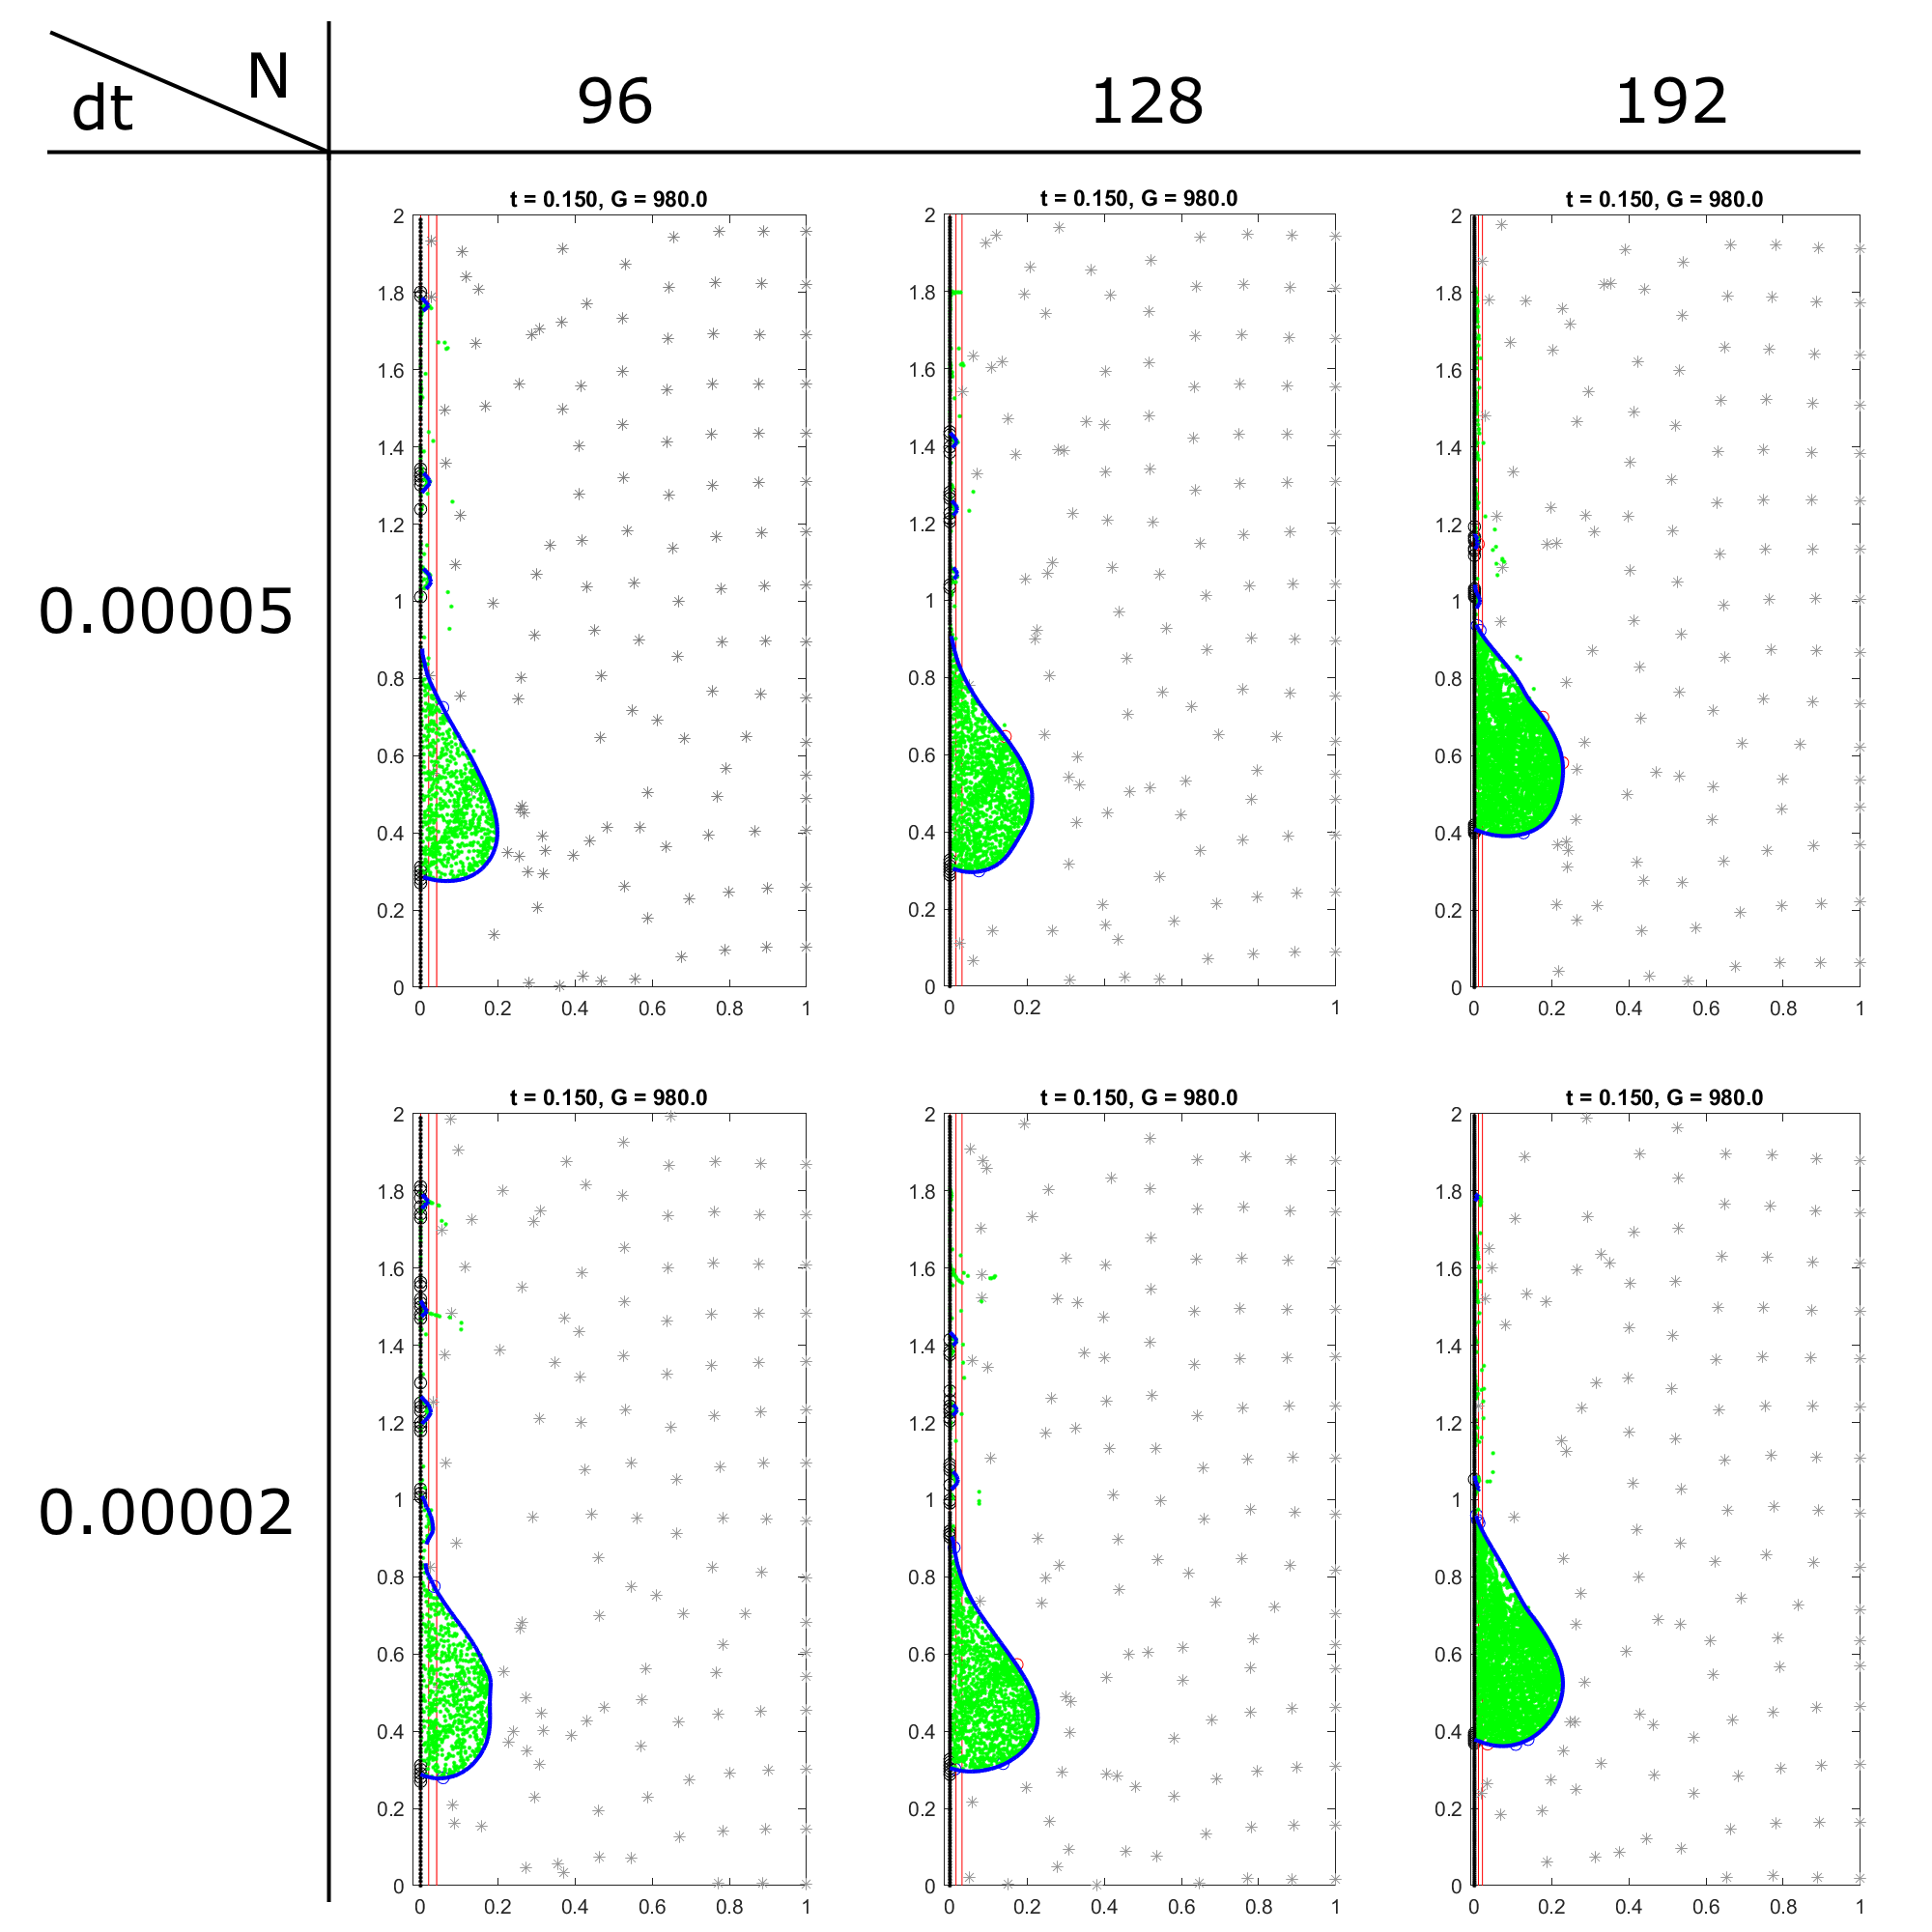
\includegraphics[scale=0.6]{figs/terminal.pdf} 
\caption{Terminal state of the sliding droplet simulation, for several different values of $dt$ and $N$. The simulation is only terminated after the droplet reaches equilibrium and stops moving. The droplet leaves a trail as it slides down the wall. From $N = 192$, further increasing $N$ yields no visible changes to the simulation video.}
\label{fig:terminal}
\end{figure}
Here we simulate a droplet sliding down a vertical wall as shown in Figure~\ref{fig:terminal}. Setup details can be found in subsection \ref{subsec:dow}. In this test case, gravity competes with the sliding friction and the upward airflow. We vary the time-step $dt$ and the spatial resolution $N$ and depict the terminal state ($t = 0.15$ s). We observe that improvement is achieved if we increase the spatial resolution $N$ to $192$. Increasing $N$ further yields no visible improvement. 

\subsubsection {Test 2: Coalescence of two droplets}
In this test case, computational domain $L=2$ cm, tension coefficient $\sigma=0.0005$ kg\,m/s$^2$, gas density $\rho_g=0.1$ g/cm$^2$, liquid density $\rho_l=1$ g/cm$^2$, and viscosity $\mu=0.01$ g/s. 
\begin{figure}
\centering
\begin{lapsetable}{6}{.1}
$N$ & $dt$ & $t$=0.01&0.02&0.03&0.04&0.05&0.06
\lapse{merge2}{0.000500}{64} {\scinote{5}{-4}}{6}{5.5}{4}{4.8}{1.5}
\lapse{merge2}{0.000200}{96} {\scinote{2}{-4}}{6}{5.5}{4}{4.8}{1.5}
\lapse{merge2}{0.000100}{128}{\scinote{1}{-4}}{6}{5.5}{4}{4.8}{1.5}
\end{lapsetable}
\caption{Two droplets coalesce with three levels of resolution refinement. Little improvement is gained from $N = 96$ to $N = 128$, rendering $N = 128$ high enough (holding other parameters constant) for demanding test cases such as this.}
\label{fig:merge_two}
\end{figure}
Here we simulate two droplets coalescing as shown in Figure~\ref{fig:merge_two}. The coalescence of two droplets is an extremely challenging test case since the coalescing moment amplifies previous perturbations. Using our surface tension model and interface splicing techniques, the simulation results show good spatial and temporal convergence.

\subsubsection {Test 3: Coalescence of six droplets}
In this test case, computational domain $L=2$ cm, tension coefficient $\sigma=0.0005$ kg\,m/s$^2$, gas density $\rho_g=0.1$ g/cm$^2$, liquid density $\rho_l=1$ g/cm$^2$, and viscosity $\mu=0.01$ g/s. 

\begin{figure}
\centering
\begin{lapsetable}{6}{.13}
$N$ & $dt$ & $t$=0.01&0.02&0.03&0.04&0.05&0.06
\lapse{merge6}{0.000200}{96} {\scinote{2}{-4}}{6}{3.4}{3.8}{2.3}{1.5}
\lapse{merge6}{0.000100}{128}{\scinote{1}{-4}}{6}{3.4}{3.8}{2.3}{1.5}
\lapse{merge6}{0.000050}{192}{\scinote{5}{-5}}{6}{3.4}{3.8}{2.3}{1.5}
\end{lapsetable}
\caption{Two droplets coalesce with three levels of resolution refinement. Little improvement is gained from $N = 128$ to $N = 192$, rendering $N = 192$ high enough (holding other parameters constant) for demanding test cases such as this.}
\label{fig:merge_six}
\end{figure}
Here we simulate six droplets coalescing as shown in Figure~\ref{fig:merge_siz}. The six-droplet coalescence test is even more challenging, since the system's response to the first coalescence event is amplified by the successive coalescence events. Our system demonstrates an interesting property that although high $dt$ leads to instability issues, but once the instability is resolved, slowly lowering $dt$ leads to fast convergence and high accuracy. 

\subsubsection {Test 4: Letters "IB" fall into an elastic pouch}
\label{subsubsec:letters}
In this test case, computational domain $L=10$ cm, tension coefficient $\sigma=0.0005$ kg\,m/s$^2$, gas density $\rho_g=0.1$ g/cm$^2$, liquid density $\rho_l=1$ g/cm$^2$, and viscosity $\mu=0.01$ g/s. 

\begin{figure}
\centering
\begin{lapsetable}{7}{.12}
$N$ & $dt$ & $t$=0&0.03&0.06&0.09&0.12&0.15&0.24
\lapse{letters}{0.0005}{96} {\scinote{5}{-4}}{7}{6}{4}{5}{5}
\lapse{letters}{0.0003}{128}{\scinote{3}{-4}}{7}{6}{4}{5}{5}
\end{lapsetable}
\caption{Letter-shaped droplets falling into elastic pouch, simulated in two resolution levels. This demos our method's capability of simulating the two-way coupling between a changing-shape solid and a two-phase fluid flow. }
\label{fig:letters}
\end{figure}
Here we initialize liquid droplets in the shape of Latin letters ``IB" and let them fall into an elastic pouch (Figure~\ref{fig:letters}). At the beginning of the simulation, the droplets change shape under surface tension, eliminating sharp corners. As the droplets hit the pouch, the pouch deforms and the gas bubbles make their way out from the liquid body. This test case demonstrates the capabilities of our method in an all-in-one setting. Note that here the solid membrane is dynamic, rendering static boundary conditions unsuitable. This shows that our methods are capable of simulating the two-way coupling between a changing-shape solid and a two-phase fluid flow, simulating surface tension, unbalanced Young stress, and solid elasticity at the same time. 

\subsection {Droplets on a wall} \label{subsec:dow}
In this section, we consider a droplet sliding down a wall. The computational domain is $1$ cm by $2$ cm. We prescribe the periodic boundary condition for the top and bottom boundaries and the symmetry boundary condition for the left and right boundaries (see \S\ref{sec:bc}). The liquid density is taken to $\rho_l=1$ g/cm$^2$ and the gas density $\rho_g=0.1$ g/cm$^2$. Viscosity for both the liquid and gas phases $\mu=0.01$ g/s. The surface tension coefficient $\sigma=0.0005$ kg\,m/s$^2$ and gravitational acceleration $g=980$ cm/s$^2$. 
    % \charles{do we have a reference or refs for these values?} \daniel{no, since 2D is inherently fictional}
    
There is a vertical wall at $x=0$ and its minimum static friction $f_\text{min}=25$ N. There is an upward vertical gas flow of $30$ cm/s, prescribed onto the velocity field at $y=0$. The prescribed velocity diminishes as $x$ approaches $0$. Specifically, at $(x,0)$, the fluid vertical velocity is $tanh(4x / L)$. 
    
\subsubsection {Effects of droplet size}
\begin{figure}
\centering
\begin{shortlapsetable}{6}{.08}
Diameter & $t$=0&0.02&0.04&0.06&0.08&0.10
\tabularnewline 0.4
\lapseShort{size_effect/output_0.400000}{6}{5}{4}{8.5}{2}
\tabularnewline 0.5
\lapseShort{size_effect/output_0.500000}{6}{5}{4}{8.5}{2}
\tabularnewline 0.6
\lapseShort{size_effect/output_0.600000}{6}{5}{4}{8.5}{2}
\end{shortlapsetable}
\caption{Bigger droplets slide faster due to gravity.}
\label{fig:droplet_size}
\end{figure}
In Figure~\ref{fig:droplet_size} we vary the size of the droplet to study the response. Observe that the smaller droplets do not slide down; rather, they obey the ``no slip" rule. This aligns with reality and is implemented with the "no slip" term in our MCL model (see \S\ref{subsec:mcl}). In the meantime, we tell the program to track the wall markers that are vertically displaced by our MCL model at every time-step. We observe that vertical displacement only happens near the contact point (usually within 6 to 8 cells). This means that although our MCL model applies to the entire wall, the majority sections of the wall are as though they were no-slip. This is consistent with previous literature that tangential viscous stress is not enough to incur apparent slip in subsonic flows with hydrophilic surfaces \citep{MD_navier}. The unbalanced Young force is the dominating tangential force near the contact point. 

\subsubsection {Big droplet catches up with small droplet}
\begin{figure}
\centering
\begin{shortlapsetable}{8}{.12}
$t$=&0.01&0.02&0.03&0.04&0.05&0.06&0.07&0.08
\tabularnewline
\lapseShort{big_chase_small}{8}{5}{4}{8.5}{1.4}
\end{shortlapsetable}
\caption{A big droplet catches up with a smaller droplet and coalesces with it.}
\label{fig:big_chase_small}
\end{figure}
In Figure~\ref{fig:big_chase_small} we initialize two droplets of different sizes on the wall. This test case shows the system's response to droplet size in one simulation and, at the same time, demonstrates the interface splicing capabilities near the wall. 

\subsection {Performance of the re-sampling technique} \label{subsec:resample}
\begin{figure}
\centering
\begin{shortlapsetable}{3}{.23}
Re-sample & $t$ = 0.028&0.045&0.078
\tabularnewline Off
\lapseShort{resample/bad}{3}{7}{4}{8.5}{5}
\tabularnewline On
\lapseShort{resample/good}{3}{7}{4}{8.5}{5}
\end{shortlapsetable}
\caption{As fluid flow advects the interface markers, if the re-sampling step is turned off, then the interface breaks into pieces and the holes start to allow flux.}
\label{fig:resample_comp}
\end{figure}
Figure~\ref{fig:resample_comp} shows a comparison study on the effect of our step-wise re-sampling technique. In the upper row, we do not re-sample, resulting in badly distributed Lagrangian markers and, eventually, topological errors. On the lower row, adding the re-sampling technique fixes the problem. 

\subsection {Demos of interface splicing}
\begin{figure}
\centering
\begin{shortlapsetable}{7}{.13}
$t$=&0.187&0.190&0.193&0.197&0.2&0.103&0.207
\tabularnewline
\lapseShort{split}{7}{6.4}{4.2}{4.6}{4.8}
\end{shortlapsetable}
\caption{A droplet splits into two.}
\label{fig:split}
\end{figure}
In Figure~\ref{fig:split}, a droplet separates into two smaller ones. After the splicing moment, surface tension quickly brings the sharp edge into the body of the droplet. During that process, the surface length of the droplet drastically shrinks, posing a challenge to the interface re-sampling algorithm. Because the edge is sharp, the rapid removal of markers leads to a spurious loss of tension energy. In future works, this can be remedied with an improved interface re-sampling algorithm where the sharpness of edges are checked and blunt areas are prioritized for re-sampling. 
    
\begin{figure}
\centering
\begin{shortlapsetable}{8}{.09}
$t$=&0.019&0.021&0.022&0.024&0.027&0.029&0.035&0.040
\tabularnewline
\lapseShort{wall_merge}{8}{5}{4.8}{9.5}{3.5}
\end{shortlapsetable}
\caption{Two droplets merge on the wall.}
\label{fig:wall_merge}
\end{figure}
In Figure~\ref{fig:wall_merge}, two droplets coalesce on the wall. This is one of the six basic cases of interface splicing. 
    
% \subsection {Energy and Area Conservation}
%     \daniel{I can track the energy error from interface re-sampling and splicing.}
%     \daniel{Do it!}
%     \daniel{But I did not keep the plotting script QAQ}

% \subsection {Spurious Currents}
%     [compare shrink]
%     \daniel{Do we even include this part? I think Puelz once said this is just well-known for IB methods.}

% \subsection {Computation Costs and Instability Issues}
%     \begin{figure}
%         \begin{subfigure}{.5\textwidth}
%         \centering
%         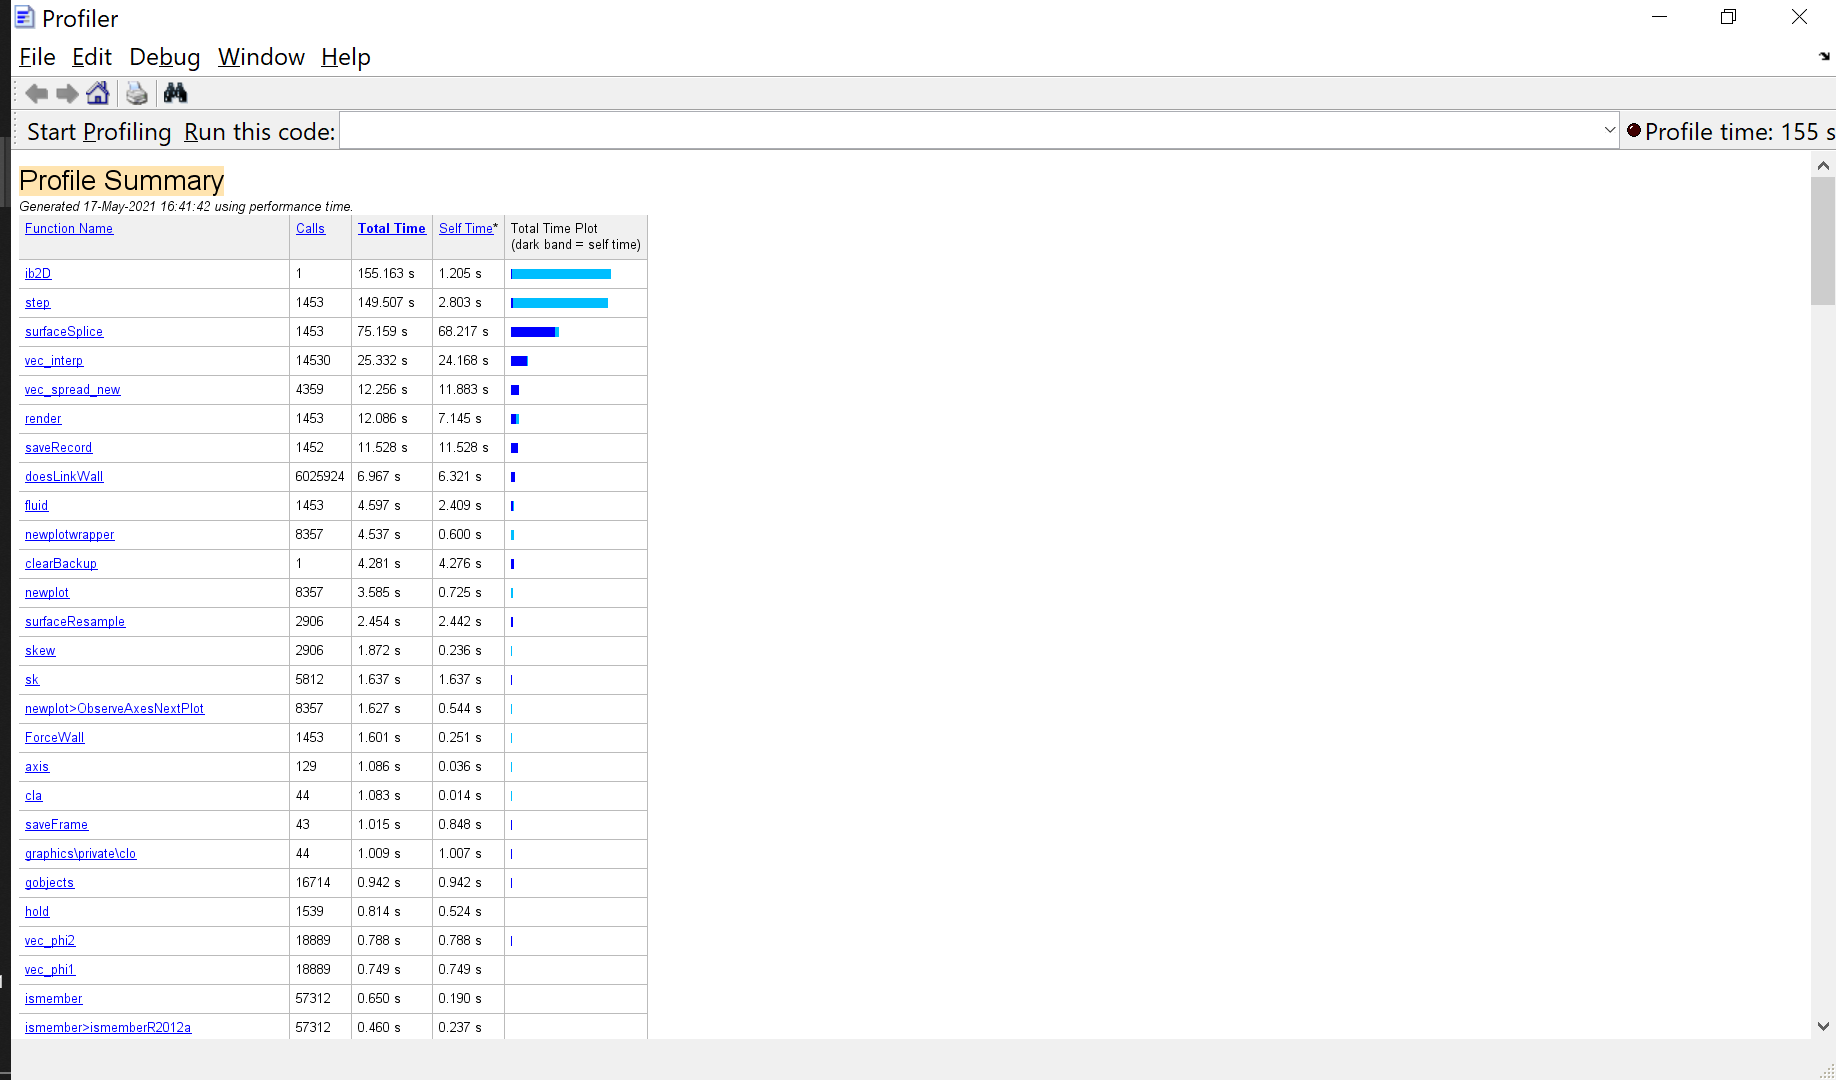
\includegraphics[width=\textwidth,trim={0mm 0mm 0mm 0mm},clip]{figs/time_profiling/summary.pdf}
%         \end{subfigure}
%         \begin{subfigure}{.5\textwidth}
%         \centering
%         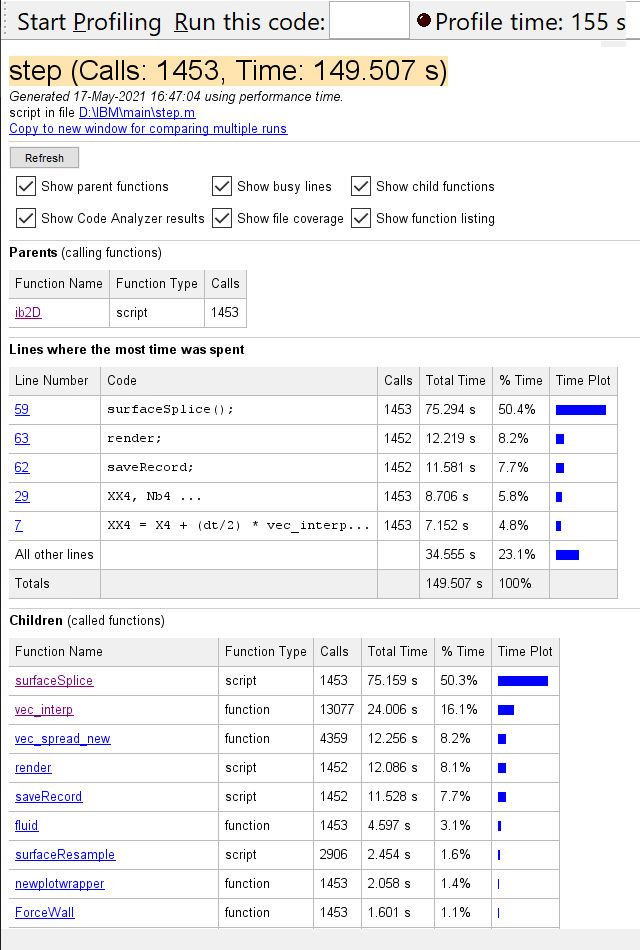
\includegraphics[width=\textwidth,trim={0mm 0mm 0mm 0mm},clip]{figs/time_profiling/step.pdf}
%         \end{subfigure}
%         \\
%         \begin{subfigure}{.36\textwidth}
%         \centering
%         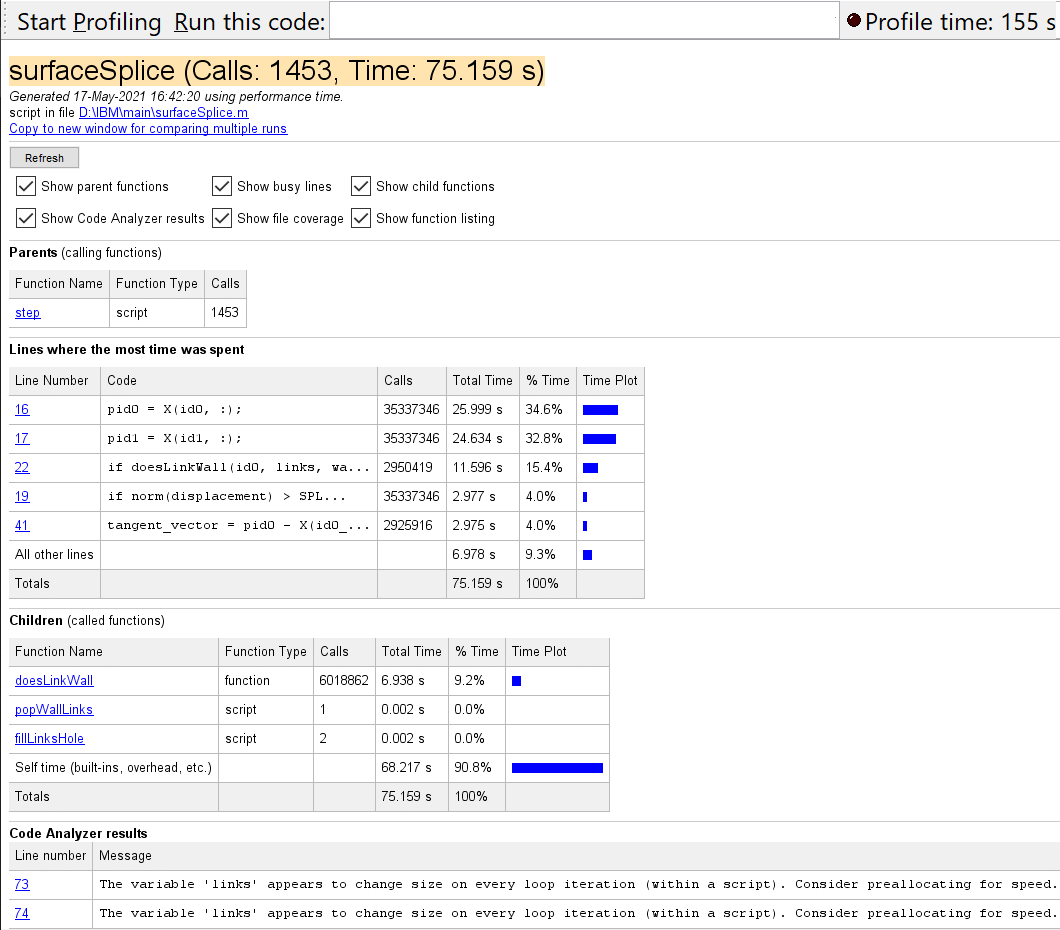
\includegraphics[width=8cm,trim={0mm 0mm 0mm 0mm},clip]{figs/time_profiling/surfaceSplice.pdf}
%         \end{subfigure}
%         \begin{subfigure}{.64\textwidth}
%         \centering
%         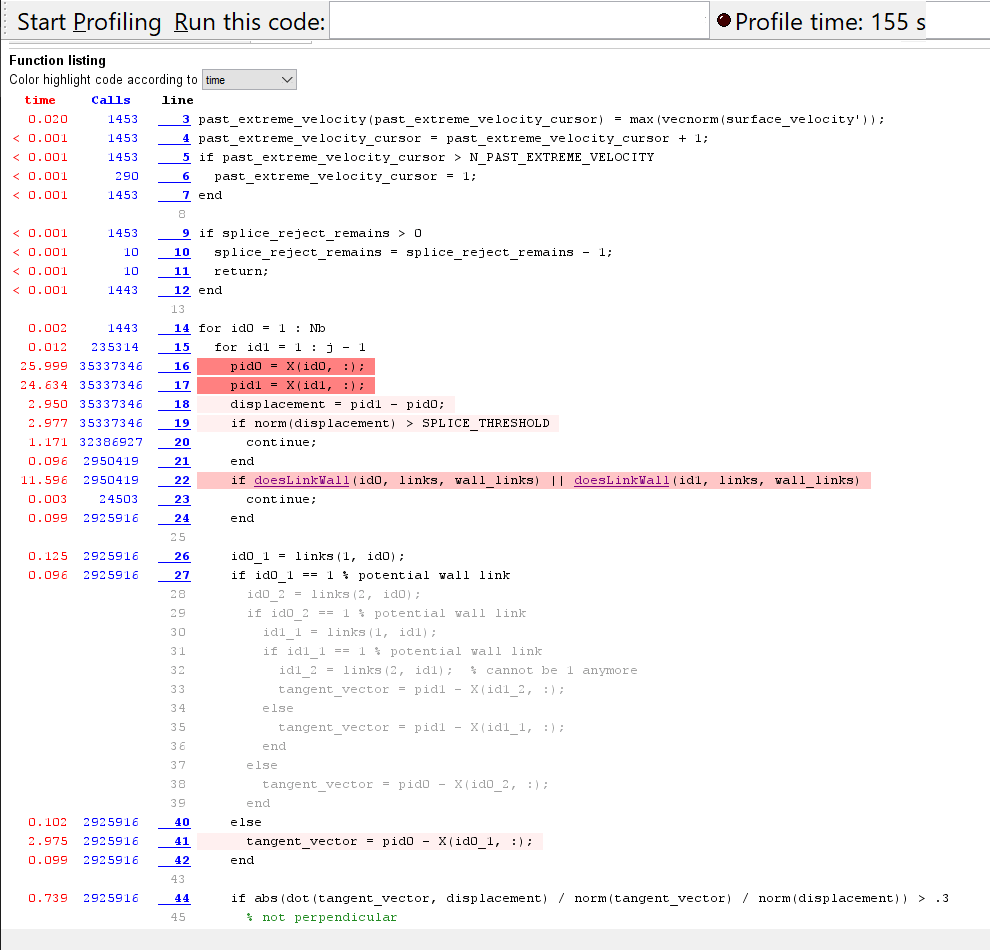
\includegraphics[width=\textwidth,trim={0mm 0mm 0mm 0mm},clip]{figs/time_profiling/code.pdf}
%         \end{subfigure}
%         \caption{
%             Matlab profiler showing the time consumption at each step of the simulation. Interface splicing is the most expensive computation. 
%         }
%         \label{fig:computation}
%     \end{figure}

%     Figure \ref{fig:computation} shows the time consumption of various computations involved in our method. The most expensive computation out of the box is interface splicing. This is due to its $O(N^2)$ nature. Despite the optimization tricks mentioned in \ref{subsec:splice}, it is still the main cost of simulation. The second slowest operation is the vector interpolation for the variable density \citep{IBM_variable_density} markers. Spreading the 2D soup of markers to the Eulerian grid is expensive. The rest of the operations are in the same timescale with the vanilla IB method. 
    
%     The existence of surface tension poses a stiffness problem. $dt$ has to be very small to avoid instability. We also observe that, the finer the spatial resolution, the smaller the time-step needs to be. Otherwise, spurious oscillating fluid velocity will emerge and quickly drives everything to NaN. 
    
%     The interface re-sampling algorithm makes a minor contribution to the instability. This is intuitive in a sense that removing a marker forces a previously-curving surface to become straight. Although the effect is minimal, it does apply a spurious normal force to the fluid interface. This then encourage the neighboring markers to bend in the other direction, forming a zigzag pattern. In reality, this issue only occurs very rarely. 

\section{Conclusions} \label{sec:conclusion}
Limitations: incompressible. 1:1 viscousity. 
\daniel{Leave till later}

\section*{Acknowledgements} 
We thank Otto Mierka and Stefan Turek for providing the 10:10 viscosity benchmark data. Several very helpful conversations with Guanhua Sun are gratefully acknowledged. P.S. is supported by an Institutional Support of Research and Creativity (ISRC) grant provided by New York Institute of Technology and financial support from the National
Science Foundation (NSF) under Grants No. DMS-2108161. 

\section{Appendices} 
\subsection{Analytical modelling of the hanging droplet equilibrium} \label{app:equi}
    The shape of the hanging droplet is determined by the following equations:\\
    \begin{equation}
        \vec{g}=g\cdot\hat{j}, \quad
        \nabla{p}=\rho\cdot{g}, \quad
        \frac{\mathrm{d}p}{\mathrm{d}y}=-\rho\cdot{g}, \quad
        p=-\rho\cdot{g}\cdot{y}+p_{\text{const.}}
    \end{equation}
    At the interface, we define the surface tension as:\\
    \begin{equation}
        p=p_{a}+\sigma \cdot \kappa(s),
        \label{eq:pressure}
    \end{equation}
    where $p_{a}$ is the air pressure, and $\kappa(s)$ is the surface curvature. By parametrization of the surface, we get:\\
    \begin{align}
        r(s)=x(s)\cdot\hat{i}&+y(s)\cdot\hat{j}.\\
        \hat{t}=\frac{\mathrm{d}r}{\mathrm{d}s}=x(s)'\cdot\hat{i}&+y(s)'\cdot\hat{j}.
    \end{align}
    We normalize the derivative by writing $1=\left(\frac{\mathrm{d}x}{\mathrm{d}s}\right)^2+\left(\frac{\mathrm{d}y}{\mathrm{d}s}\right)^2$. We get $\left|\frac{\mathrm{d}x}{\mathrm{d}s}\right|=\sqrt{(x')^2+(y')^2}=1$\\
    We define the normal vector as\\
    \begin{center}
        $\hat{n}=\hat{t}\times\hat{k}=y'(s)\hat{i}-x'(s)\hat{j}$.
    \end{center}
    Now we have a system of ODEs:\\
    \begin{equation}
        \frac{\mathrm{d}\hat{t}}{\mathrm{d}s}=-x\hat{n}(s), \quad
        \frac{\mathrm{d}\hat{n}}{\mathrm{d}s}=x\hat{t}.
    \end{equation}
    By some algebra, we get\\
    \begin{center}
        $x''(s)\hat{i}+y''\hat{j}=-x\hat{n}$.
    \end{center}
    Multiply both sides by $\hat{n}$, we get\\
    \begin{equation}
        -x=y'x''-x'y''. 
        \label{eq:curvature}
    \end{equation}
    The above equation is the curvature expression for our reparametrization.\\
    Plug \ref{eq:curvature} into \ref{eq:pressure}, we get\\
    \begin{align}
        p-\rho\cdot{g}\cdot{y(s)}&=p_{a}+\sigma(x'y''-y'x'')\\
        x'y''-y'x''+\frac{\rho\cdot{g}}{\sigma}y&=\frac{\Delta{p}}{\sigma}.
    \end{align}
    Define the capillary length $l=\sqrt{\frac{\sigma}{\rho\cdot{g}}}$,
    and by rescaling, we get\\
    \begin{center}
        $x'y''-y'x''+\frac{u}{l^2}=\frac{\Delta{p}}{\sigma}$.
    \end{center}
    Rescaling $x$, $y$ and $s$ in terms of $l$, we get\\
    \begin{center}
        $\bar{x}=\frac{x}{l}$, \quad $\bar{y}=\frac{y}{l}$, \quad $\bar{s}=\frac{s}{l}$, \quad $\Pi=\frac{l\Delta P}{\sigma}$.
    \end{center}
    We rewrite the equation in dimensionless form\\
    \begin{equation}
        x'y''-y'x''+y=\Pi.
    \end{equation}
    Without loss of generality, set initial conditions $x(0)=y(0)=0$. The first order initial conditions can be described by the contact angle $\theta$: 
    \begin{equation}
        \begin{cases}
            x'(0)=\sin(\theta)\\
            y'(0)=\cos(\theta).
        \end{cases}
    \end{equation}
    
    The above model describes the hydro-static equilibrium shape of a droplet hanging on a vertical wall as a PDE in the Cartesian space. The result shows that there is a linear relationship between the local curvature of the interface and the altitude. 

\bibliographystyle{jfm}
\bibliography{mybibfile}
% \begin{thebibliography}{99}

% \bibitem[Sanaei {\it et al.}(2016)]{Sanaei2016}
% {\sc Sanaei, P., Richardson, G.W., Witelski, T., Cummings, L.J.,}
% Flow and Fouling in a Pleated Membrane Filter.
% {\it J. Fluid Mechanics.} {\bf 795}, 36-59 (2016).

% \bibitem[Sanaei {\it et al.}(2017)]{Sanaei2017}
% {\sc Sanaei, P., Cummings, L.J.,}
% Flow and fouling in membrane filters: Effects of membrane morphology.
% {\it published at J. Fluid Mechanics.} (2017)

% %\bibitem[Sanaei {\it et al.}(2017)]{Sanaei2017cake}
% %{\sc Sanaei, P., Cummings, L.J.,}
% %Optimum Permeability Profile and Fouling in Membrane Filters.
% %{\it Preprint.}

% \end{thebibliography}

\end{document}             % End of document.
